\documentclass[11pt,a4paper]{article}
\usepackage{fontspec}
\usepackage[margin=25mm]{geometry}
\usepackage{amsmath,amssymb,booktabs,array,graphicx}
\usepackage{microtype,xcolor}
\usepackage[hidelinks]{hyperref}
\usepackage{xurl}
\setlength{\emergencystretch}{2em}
\newcommand{\pending}[1]{\textcolor{red!60!black}{[Pending: #1]}}
\newcommand{\Wall}{81.959}
\newcommand{\CPU}{81.472}
\newcommand{\RSS}{273.05}
\newcommand{\Output}{84.65}
\newcommand{\CandidateThreshold}{40.81854}
\newcommand{\RelativeIncrease}{13.30}

\title{When Should a Digital-Twin Alarm Clear?\\Recovery Evidence under Motion-Model Mismatch}
\author{Muhammad Usman \and Haiqa Mushtaq}
\date{Research draft for author review --- 17 October 2026}
\begin{document}
\maketitle
\noindent\textbf{Draft status.} This manuscript reports completed, fully synthetic experiments. It does not establish a new algorithm or reproduce the headline results of a published detector. Its primary improvement hypothesis failed. Muhammad Usman's supplied university affiliation is recorded in the declarations. Other personal declarations and approval by both authors remain unconfirmed. This draft has not been submitted or externally peer reviewed.
\begin{abstract}
A small prediction residual can justify an alarm onset rule without establishing that a disturbed process has recovered. We investigate this distinction in digital-twin motion monitoring with protected command context. A corrected observer supplies prospective residuals, while an uncorrected nominal trajectory supplies a separate return criterion. The candidate retains an alarm until measured joint state lies within a fixed reference tolerance, including a noise margin, for ten samples. We test this engineering combination against saved autoregressive predictors, rolling means, CUSUM, ordinary hysteresis, command resets and component removals. Configurations and thresholds were frozen before generating 144 episodes with new multisine and chirp commands, independently varied plant parameters, actuator lag and sensor noise. All 23 methods were scored before joint outcome inspection. The candidate overlapped all 90 interventions and had no premature clearing under the declared physical-return diagnostic, but alarmed on 2,778 of 59,400 benign observations, versus 2,452 for fused hysteresis. Its predeclared improvement criterion therefore failed. At identical entry thresholds, removing the recovery dwell caused premature clearing in 44 events; removing reference-based entry changed no alarm decision. These results distinguish a useful recovery component from an unsupported overall improvement. They also show why command-interval F1, benign alarm burden and physical-return behavior must be reported separately. Conclusions apply to the stated virtual model and trust assumptions; algorithmic novelty and real-system validity remain unestablished.
\end{abstract}
\noindent\textbf{Keywords:} digital twin; robotic motion; anomaly detection; alarm recovery; model mismatch; cybersecurity; simulation.
\section{Problem and study contribution}
Robotic motion monitoring needs to distinguish a commanded change from an unauthorized deviation. It also needs a defensible rule for ending an alarm. A predictor can track disturbed measurements well enough to produce a small residual while the process remains displaced from the approved trajectory. Conversely, a nominal reference can retain evidence of that displacement but disagree with legitimate motion when its plant model is inaccurate. This study examines the resulting detection--recovery trade-off under an explicit command-trust assumption.

Our research question is whether a separate return criterion can retain evidence until physical recovery while reducing alarms during legitimate command changes under model mismatch. We test a fixed-return rule selected from earlier development simulations. The distinction between entry and return is operational: entry uses normalized prediction discrepancy; return uses proximity to an approved-command reference, rather than a fraction of the alarm-entry threshold. Neither distinction by itself establishes novelty.

The contribution of the present experiment is a falsifiable test of that mechanism, including controls that receive the same protected context, component removals at both normal-calibrated and identical entry thresholds, and a fresh condition matrix frozen before its outcomes existed. The resulting evidence identifies which component changes recovery and where the overall improvement fails. It does not support a claim that the candidate is a superior detector or an original replacement for existing observer-based diagnosis. The longer-term original-method contribution remains a research objective, rather than a conclusion of this draft.

\section{Related work and comparator scope}
CASPER uses external inertial measurements to monitor robotic motion and studies anomalies introduced through joint-velocity changes \cite{casper}. Its corrected version of record is an ACM Transactions on Internet of Things article; the correction date is distinct from the original 2024 publication. The later edge-computing study investigates real-time robotic-arm anomaly detection \cite{edge}. These papers motivate the concern that a learned predictor and its scoring history may respond differently to brief and persistent deviations. They do not supply an interchangeable benchmark for our four-channel joint-state simulation. Previously saved nine-channel IMU CNNs belong to a separate recorded-data track; no input conversion or claim of paper-faithful reproduction is made here.

TWINE integrates a manufacturing digital-twin framework with explainable anomaly detection \cite{twine}. Its accepted manuscript is available in the author's institutional repository. The inspected supervised classification workflow has different label access from the normal-only procedure used here. Ayankoso et al. combine trajectory-change recognition with condition monitoring \cite{ayankoso}; this is relevant to legitimate motion variation, but does not establish that a change in observed trajectory is authorized. These differences require explicit admission decisions rather than a ranking assembled from published scores.

The methodological background is broader than recent robotic cybersecurity papers. Interval-observer diagnosis already treats the interaction of observer gain, uncertainty and fault sensitivity \cite{meseguer}. CUSUM is an established accumulated-deviation control \cite{nist}. Our three-model envelope, dwell counter and residual fusion therefore receive ordinary-control status. A sampled envelope is not a verified enclosure of all admissible dynamics.

Two recent leads further restrict novelty claims. Ahmed et al. describe a robust adaptive propagated interval observer for actuator-fault diagnosis \cite{rapio}; publisher-indexed information was accessible, but complete recovery equations and matched code remain unverified. Kaisar et al. describe digital-twin-based false-data-injection detection and isolation in robotic vehicles \cite{kaisar}; institutional abstract and bibliographic metadata were verified, but the full manuscript was unavailable to this audit. We do not infer exact equivalence or superiority from these partial records. Their overlap with uncertainty handling and recovery is sufficient to prevent a first-of-its-kind claim until the full comparison is resolved.

The experimental roster consequently consists of transparent controls and our specified candidate, not three faithful recent-paper reproductions. Public voraus-AD recordings are a promising separate source of robot fault observations \cite{voraus}. Their verified availability does not establish an authenticated approved-command channel or the physical-return annotation required by this particular question. No independent recording is silently substituted into the present confirmation.

\section{Virtual plant, information and threat model}
The simulated plant is a horizontal two-revolute-joint arm with point masses. Its state is $x=[q_1,q_2,\dot q_1,\dot q_2]^\top$, with angles in radians and time in seconds. Writing $a=m_2l_1l_2$ and $d=m_2l_2^2$, the mechanical equations are
\begin{align}
 M(q)\ddot q+c(q,\dot q)+B\dot q&=\tau,\\
 M(q)&=\begin{bmatrix}
 (m_1+m_2)l_1^2+d+2a\cos q_2 & d+a\cos q_2\\
 d+a\cos q_2 & d
 \end{bmatrix},\\
 c(q,\dot q)&=a\sin q_2\begin{bmatrix}-2\dot q_1\dot q_2-\dot q_2^2\\\dot q_1^2\end{bmatrix}.
\end{align}
Nominal parameters are $m_1=1$, $m_2=0.8$ kg, $l_1=0.5$, $l_2=0.4$ m and $B=\operatorname{diag}(0.08,0.06)$. A saturated proportional--derivative controller requests
\begin{equation}
 \tau^*=\operatorname{clip}\{K_p(q^c-q)+K_d(\dot q^c-\dot q),-20,20\},
\end{equation}
componentwise, with $K_p=\operatorname{diag}(18,12)$ and $K_d=\operatorname{diag}(4,3)$. For a lagged plant, actuator torque is an additional two-dimensional state satisfying $\dot\tau=(\tau^*-\tau)/T_a$. The zero-lag plant applies $\tau^*$ directly. The monitor retains the lag-free nominal model in every condition. Gravity, contact, flexible links, thermal effects, communication jitter and actuator faults beyond the declared command manipulations are absent.

The plant receives an executed command $u^e=[q^c,\dot q^c]$. The monitor receives a protected approved command $u^a$, a context-validity flag and noisy truthful joint measurements $y=x+\epsilon$. Nominal independent Gaussian sensor standard deviations are $(0.0005,0.0005,0.002,0.002)$. Plant-specific noise scaling is stated below. The attacker changes the downstream executed command without changing the protected approved record or measurement stream. Authorized changes update both command paths. This separates the effect of permission context from the physical shape of a change. Authentication itself is assumed, not implemented or demonstrated.

The detector API excludes executed commands, true states, actual plant parameters, scenario names, intervention schedules and labels. When context is unavailable, the command channel holds its last available value. Context-dependent decisions become unknown. A stateful alarm remains internally latched and its recovery counter resets; unknown observations do not become known negatives. Context-free persistence and AR remain available. The attack model excludes coordinated compromise of the protected command and all sensing channels. The experiment cannot establish security under that stronger adversary or distinguish every mechanical fault from malicious intent.

\section{Prediction and recovery mechanisms}
Let $F_0$ be one nominal integration step and $r_t$ a reference driven by the available approved command. A following observer maintains a separate estimate $\hat x_t^-$. Its recursion is
\begin{align}
 r_{t+1}&=F_0(r_t,u_t^a),\\
 \hat x_{t+1}^-&=F_0\{\hat x_t^-+L(y_t-\hat x_t^-),u_t^a\},
 \qquad L=\operatorname{diag}(0.65,0.65,0.35,0.35).
\end{align}
Scores at $t$ use $\hat x_t^-$ before the current measurement corrects the state. Both trajectories begin at the declared task's initial pose and zero velocity. Parameters, gains and residual scales remain fixed throughout an episode. This supplies explicit state correspondence and prospective prediction in software; it does not demonstrate synchronization with a real robot.

With training standard deviation vector $s$, define
\begin{equation}
 e_t^f=\tfrac14\sum_{j=1}^{4}[(y_{t,j}-\hat x^-_{t,j})/s_j]^2,
 \qquad
 e_t^r=\tfrac14\sum_{j=1}^{4}[(y_{t,j}-r_{t,j})/s_j]^2.
\end{equation}
Training means $\bar e^f,\bar e^r$ normalize a fused entry score
\begin{equation}
 z_t=\max(e_t^f/\bar e^f,e_t^r/\bar e^r).
\end{equation}
Ordinary fused hysteresis enters when $z_t>h$ and clears after ten valid consecutive samples at $z_t\le h/2$. An above-threshold observation has priority and restarts the recovery count. An earlier two-evidence proposal reduces exactly to this maximum-score hysteresis; it is retained as a classical comparator.

The fixed-return candidate uses the same entry score but replaces the low-score condition by
\begin{equation}\label{eq:return}
 R_t=\mathbf 1\!\left\{\forall j:\ |y_{t,j}-r_{t,j}|+3\sigma_j\le0.1s_j\right\}.
\end{equation}
After entry, the candidate clears when $R_t=1$ for ten consecutive valid observations without a new entry. The ten-observation window spans nine sample intervals; we report the count explicitly rather than calling it an exact 0.20 s residence time. The $3\sigma$ allowance is a design margin, not a deterministic bound on Gaussian noise or a confidence certificate. In the noisy fresh plant the detector still uses its original nominal $\sigma$.

The saved AR(4) and ARX(4) controls predict standardized state using four preceding observations; ARX also receives the preceding approved command. They use ridge coefficient $0.001$ with an unpenalized intercept. Persistence uses the preceding observation. Their scores are channel-mean squared standardized errors. A 45-sample trailing mean and a CUSUM operate on following-observer error. The latter obeys
\begin{equation}
 C_t=\max\{0,C_{t-1}+\min(e_t^f/\bar e^f,25)-1.5\}.
\end{equation}
Its cap and drift are fixed experimental settings, not an optimized implementation of a published paper.

Additional controls include mode-conditioned fusion, an envelope from three nominal-model parameter combinations, and their ordinary or fixed-return decisions. The envelope score is the maximum per-channel excess outside the sampled trajectory range divided by nominal sensor noise. Mode conditioning uses protected command increments to flag a 50-sample transition interval and fixed training normalizers. A command-reset control clears ordinary fused hysteresis at the start of a detected command-mode interval, before applying the current entry rule; it never receives an intervention boundary.

Six added normal-calibrated variants remove the dwell, remove the noise margin, use reference-only entry, use following-only entry, add following-error hysteresis, or apply the command reset. Removing reference entry retains the reference in the return test. Four further ablations retain the candidate's identical $h$ while changing only its decision rule to point thresholding, ordinary hysteresis, one-sample return or zero-margin return. This second track isolates the return mechanism; its members need not have the same calibration alarm burden. All 23 definitions and exact thresholds are retained in the code and appendix.

\section{Frozen evaluation design}
\subsection{Development, calibration and fresh conditions}
Earlier simulation cycles were exposed development evidence. The immediately preceding cycle tested 144 episodes with thirteen methods. Its envelope candidate missed the complete predeclared improvement target and showed substantial extrapolation failure. A simpler fixed-return ablation was the stronger within-range development lead. We selected that ablation before generating the present data; no finding from this cycle selected its configuration.

All fitted coefficients, channel transforms, residual means and mode normalizers were retained from the earlier normal-only study. Eighteen normal calibration episodes provide 16,200 eligible targets. The first thirteen methods retain their exact saved thresholds. Each of six new normal-calibrated methods selects the smallest observed score-grid threshold, including zero and warmup scores, yielding at most 162 eligible normal alarms under its complete decision state machine. Alarms use strict exceedance. The four matched-entry diagnostics instead inherit the candidate threshold, $h=\CandidateThreshold$, without recalibration. The candidate produced 153 calibration alarms; the matched point, hysteresis, no-dwell and no-margin variants produced 4, 65, 44 and 72, respectively. Equal entry thresholds and equal alarm budgets are different experimental controls.

The fresh matrix reserves two analytic tasks. For phase $\theta(s)$, amplitudes $a_1,a_2$ and offset $\phi$, desired positions are
\begin{equation}
 q_1^c=a_1\sin\theta+0.06\sin2\theta,\qquad
 q_2^c=a_2\sin(\theta+\phi)+0.04\sin3\theta.
\end{equation}
Task C uses $\theta=0.75s+0.10\sin(0.2s)$, amplitudes $(0.28,0.38)$ and $\phi=0.55$. Task D uses $\theta=0.45s+0.0125s^2$, amplitudes $(0.33,0.42)$ and $\phi=1.05$. Velocities are analytic derivatives multiplied by the current time-warp rate. Slow commands integrate rate $0.5$ causally. An authorized slowdown retains its accrued phase delay; an unauthorized slowdown rejoins the original approved schedule when command corruption ends. That restoration can create a command discontinuity, which is part of the specified model.

\begin{table}[htbp]\centering\small
\caption{Fresh actual plants. Factors multiply nominal parameters; the monitor is unchanged.}
\begin{tabular}{lcccr}\toprule
Plant & Mass factors $(m_1,m_2)$ & Damping factors & Lag (s) & Noise factor\\\midrule
P1 & $(0.92,1.08)$ & $(1.4,0.7)$ & 0 & 1.0\\
P2 & $(1.18,0.90)$ & $(0.7,1.3)$ & 0.04 & 1.0\\
P3 & $(0.82,1.22)$ & $(1.5,0.6)$ & 0.08 & 1.5\\\bottomrule
\end{tabular}\label{tab:plants}
\end{table}

Each task--plant pair receives noise seeds 17, 42 and 2026, offset by a fixed task/plant formula before generation. Noise is paired across conditions. Eight conditions comprise unchanged motion, authorized offset, authorized slowdown, brief unauthorized offset, persistent unauthorized offset, hold, unauthorized slowdown and an offset with missing command context. Offset magnitude is $-0.18$ rad on joint 1. Interventions start at sample 350; the brief one lasts eight samples (0.16 s), while others end before sample 550. Missing context occupies samples 350--409. Each episode has 1,200 samples at 50 Hz, with the first 100 processed but excluded from metrics. State resets only between independent simulated episodes, never at labels.

The total is $2\times3\times3\times8=144$ episodes, 158,400 eligible observations per method, 59,400 observations in wholly benign episodes and 90 intervention events. These are paired virtual conditions, not 144 independent robots. The two new motion families and torque lag provide a prospective within-simulator challenge beyond new noise seeds, but not independent physical validation. No inferential population confidence interval or seed-based significance claim is made.

\subsection{Metrics and primary criterion}
Point precision, recall and F1 use the scheduled command-corruption labels without point adjustment. Unknown decisions do not count as alarms; their positive labels remain false negatives. Average precision uses underlying scores, with unknown scores ranked below all valid scores and all positive labels retained. Consequently AP evaluates score ranking rather than the complete alarm latch. Variants sharing a score have identical AP even when their alarms differ.

Benign alarm fractions use wholly benign episodes, separating legitimate-operation burden from post-corruption recovery. Alarm episodes per eligible hour count causal rising edges; missing-context reappearance is not a fresh onset. Event overlap means at least one known alarm within the intervention. A fresh detection additionally requires a known alarm rising edge. All misses remain in event denominators; delays are conditional on the stated detected subset. An overlapping alarm alone is not proof of timely new detection.

For evaluation only, physical return is the first start of ten consecutive true-state observations within $0.1s_j$ of the nominal reference in every channel after the executed command is restored, searched within five seconds. This compares simulated state to a modeled trajectory; it is neither a damage metric nor a safety criterion. Premature clearing means an alarm falls after its first known event hit but before that declared return. Unalarmed gaps and absence of return are also preserved. Clearing delay is the first known non-alarm at or after return, up to five seconds. A method that cleared too early can therefore have zero delay: the premature-clear metric must be read alongside it.

The primary criterion requires the candidate to reduce benign alarm points by at least 25\% against \emph{both} fused hysteresis and mode-conditioned hysteresis, without more benign alarm episodes, missed overlaps, missed fresh onsets or premature-clear events. At least 95\% of detected events with a physical return must clear within five seconds. The complete conjunction was specified before generation. Subgroups and component comparisons are descriptive; they do not replace this primary outcome.

\subsection{Integrity, validation and resources}
Ten scientific source/specification files and 809 prior inputs were hash-bound before execution. Normal thresholds were sealed before fresh generation; all fresh scores were sealed before joint outcome computation. Fourteen synthetic tests cover command derivatives, lag dynamics, integration refinement, causality, unknown/reset behavior and threshold rules. A fresh-process audit then passed 14,635 checks, including unchanged fitted state, threshold replay, score/decision identities and separate contingency arithmetic. Shared-code replay and separate arithmetic are useful checks, not independent external replication.

The experiment used one supervised attempt with caps of 600 s wall time, 300 s CPU, 1 GiB monitored memory and 160 MiB outputs. It ran in an isolated Python 3.12.15/NumPy 1.26.4 environment on an Apple M5 Pro computer with 24 GiB memory. No new neural training, raw-data access or physical operation occurred. Source hashes, interpreter and dependency versions, configuration, seeds, commands, revision/dirty state and all outcomes are retained. Figures and tables are produced by a separate reporting script from saved artifacts. Codex (OpenAI, GPT-6-based agent; exact serving build unavailable) assisted research design, implementation, execution, verification and writing. Human review of those outputs remains pending and is not implied by automated checks.

\section{Results}
\subsection{Primary outcome and strong controls}
All 3,312 episode--method outcomes were preserved. The primary criterion failed. Fixed return alarmed on 2,778 benign observations (4.68\%), compared with 2,452 (4.13\%) for fused hysteresis: a \RelativeIncrease\% increase rather than the required reduction. It reduced benign points by 59.41\% against mode hysteresis, but success against only one control cannot satisfy the frozen conjunction. The candidate had 41 benign alarm episodes versus 45 for fused hysteresis and 175 for mode hysteresis. Its longer alarm time therefore did not imply more alarm episodes.

\begin{table}[htbp]\centering\small
\caption{Selected controls and candidate on the fresh pooled population. Overlap/fresh counts have denominator 90; early denotes events with premature clearing. Full roster appears in Appendix~\ref{app:all}.}
\begin{tabular}{lrrrr}
\toprule
Method & Benign (\%) & F1 & Overlap/fresh & Early \\
\midrule
ARX(4) & 6.00 & 0.644 & 90/80 & 90 \\
Rolling mean (45) & 4.43 & 0.709 & 90/72 & 87 \\
CUSUM & 44.05 & 0.216 & 81/39 & 0 \\
Following hysteresis & 2.57 & 0.795 & 90/72 & 90 \\
Fused hysteresis & 4.13 & 0.677 & 90/72 & 3 \\
Mode hysteresis & 11.52 & 0.519 & 90/72 & 0 \\
Fixed return & 4.68 & 0.650 & 90/72 & 0 \\
\bottomrule
\end{tabular}
\label{tab:main}
\end{table}

Fixed return, fused hysteresis and mode hysteresis each overlapped all 90 events and produced 72 fresh event onsets. All 18 absent fresh onsets for fixed return occurred in the missing-context condition; later known overlap did not satisfy the stricter fresh-onset definition. The candidate had no premature clears or known unalarmed gaps before declared return. Fused hysteresis had premature clearing in three events and 15 gap observations. All 90 candidate events returned and cleared within five seconds; the maximum measured clearing delay was 0.92 s. These satisfy the recovery and noninferiority clauses but do not compensate for the failed alarm-burden clause.

Following-error hysteresis was a strong ordinary control: F1 was 0.795, versus 0.650 for fixed return, with 1,529 benign alarm points. It nevertheless cleared before declared physical return in all 90 events. Its zero maximum clearing delay reflects alarms already absent at return, not a better recovery guarantee. This is the central metric conflict. Retaining evidence after command restoration counts against command-interval precision even when it aligns with the separate return diagnostic. Fixed return had 10,188 alarmed observations in the common 22,500-observation post-command windows, compared with 9,144 for fused hysteresis and 4,187 for following hysteresis.

CUSUM illustrates the opposite failure. It overlapped 81 events with 39 fresh onsets, missed nine events, and alarmed on 26,165 benign observations. None of its 81 detected-returned events cleared within the five-second window. Its memory retained evidence, but the retained burden was not selective enough for the declared task. The rolling mean remained a useful control with F1 0.709 and 2,632 benign alarm points, while showing premature clearing in 87 events. Persistence and AR had low point recall despite many event overlaps; their alarms often captured transitions rather than sustained deviation. Appendix tables retain these differences rather than filtering controls by their strongest metric.

\begin{figure}[htbp]\centering
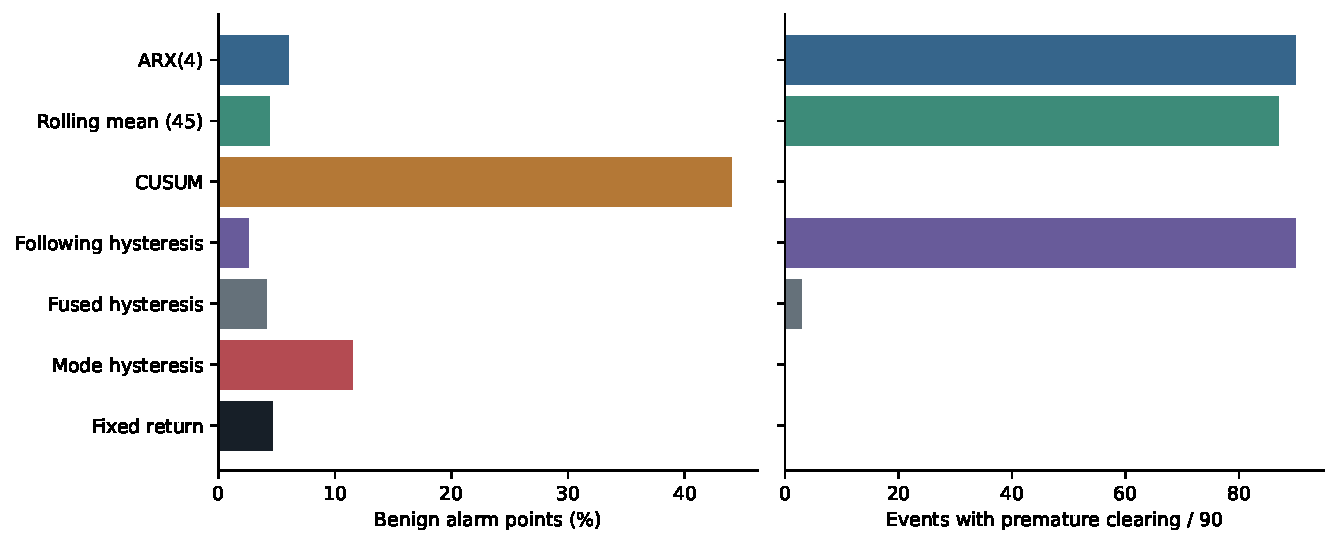
\includegraphics[width=\linewidth]{figures/tradeoff.pdf}
\caption{Benign alarm time and premature clearing describe different costs. All panels use saved pooled outcomes; zero premature clearing alone can also describe a method that remains alarmed. Figures are generated reproducibly from measured simulation artifacts.}
\label{fig:tradeoff}
\end{figure}

\subsection{What the component removals establish}
At the candidate's identical entry threshold, ordinary hysteresis had five premature-clear events, one-sample fixed return had 44, and removing the noise margin had one. The full rule had none (Table~\ref{tab:matched}). Removing the dwell reduced benign alarms from 2,778 to 1,813; removing the margin reduced them to 2,486. The recovery components therefore changed a measured trade-off. The results do not show that longer persistence is free or that the chosen margin has a guaranteed probability of containment.

\begin{table}[htbp]\centering\small
\caption{Matched-entry component study. All rows use $h=\CandidateThreshold$. These diagnostics do not have matched calibration alarm counts.}
\begin{tabular}{lrrr}
\toprule
Decision at same entry threshold & Benign points & Early clears & F1 \\
\midrule
Fixed return & 2778 & 0 & 0.650 \\
Matched point & 1430 & 90 & 0.731 \\
Matched hysteresis & 2389 & 5 & 0.680 \\
Matched no dwell & 1813 & 44 & 0.706 \\
Matched no margin & 2486 & 1 & 0.674 \\
\bottomrule
\end{tabular}
\label{tab:matched}
\end{table}

Separately calibrated removals tell a consistent but numerically distinct story. The no-dwell variant had 1,872 benign points and 44 premature-clear events; the no-margin variant had 2,488 and one. Replacing fused entry with reference-only entry yielded 2,547 benign points and no premature clearing. Replacing it with following-only entry produced exactly the same alarm and unknown arrays as the full candidate in every one of the 144 episodes. This last equality was checked sample by sample, rather than inferred from aggregate metrics. It shows no incremental value of reference-based \emph{entry} in these conditions. The reference still supplies recovery evidence, so this is not evidence that the reference can be removed entirely.

The command-reset control had the same reported aggregate outcomes as ordinary fused hysteresis. That observation does not establish that every internal state trajectory is equivalent; the code performs a different causal operation. No post-outcome threshold or variant was selected to improve the primary result.

\subsection{Dependence on the plant condition}
All four listed stateful methods produced zero benign alarms in P1. Fixed return produced 936 in P2 and 1,842 in P3, compared with 882 and 1,570 for fused hysteresis. Mode hysteresis produced 1,102 and 5,742. Thus the pooled failure against fused hysteresis was not created by a reversal in an otherwise unreported subgroup. Increasing model discrepancy and noise co-varied across these declared strata; the experiment does not isolate the causal effect of actuator lag from the independently changed masses, damping and sensor noise.

\begin{figure}[htbp]\centering
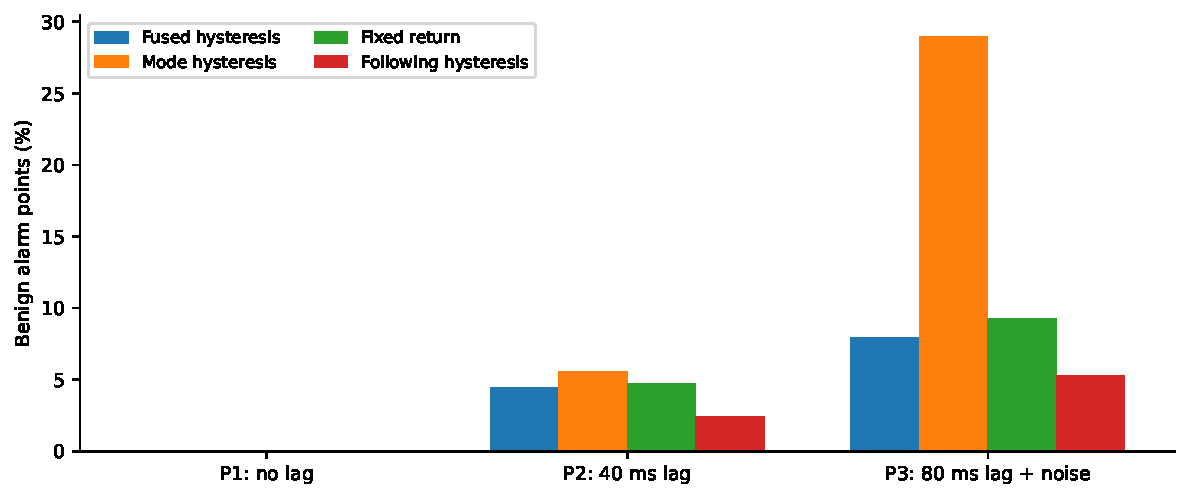
\includegraphics[width=.95\linewidth]{figures/plant_strata.pdf}
\caption{Plant-stratified benign alarm burden; each stratum contains 19,800 benign observations. Masses and damping also differ between plants, so this is not a controlled lag-only effect.}
\label{fig:strata}
\end{figure}

The earlier within-range advantage of fixed return did not carry into the new task/plant matrix as a uniform improvement. This is a prospective transfer failure within a shared simulator. It is evidence against the tested hypothesis, not a reason to relabel fresh conditions as development and omit them from the report.

\subsection{Execution cost and outcome accounting}
The supervised run completed in \Wall~s wall time and \CPU~s worker CPU time, with \RSS~MiB peak measured memory and \Output~MiB outputs. Every resource cap passed. There was one successful attempt and no scientific retry. Physical generation took 17.245~s, following-observer propagation 46.921~s, shared model-bank propagation 10.073~s and score assembly 0.627~s. These are measured component totals, not independent latency estimates for each method. Model-bank work is cached across compatible episodes and includes calibration; the separately reported calibration total overlaps some of it and must not be added again.

Candidate decision replay alone took about 11.207 ms summed across all 144 saved streams, excluding prediction and scoring. Vectorized point decisions and sequential state machines have different implementation paths, so those totals are not an embedded deployment benchmark. They establish feasibility within the stated computer budget, while the full receipts preserve the cost of shared computations.

\section{Interpretation, limitations and next evidence}
The strongest supported result is a separation of alarm entry quality from evidence for ending an alarm. At fixed entry threshold, a dwell and reference-distance condition prevented observed premature clears, while increasing benign alarm time. The command-interval ranking favored ordinary following hysteresis. A claim of overall improvement would hide one of these outcomes. The tested mechanism is useful as a diagnostic design and a controlled counterexample to treating F1 or alarm persistence alone as sufficient evidence of good recovery behavior.

This result is not a demonstrated flaw in CASPER or its successor. Those papers use different sensing modalities and their published experiments have not been faithfully reproduced here. The present classical controls were implemented explicitly to test a mechanism under common information. The earlier IMU experiments remain supporting development records, not independent confirmation of these simulated cyber conclusions. A recent-paper shortlist cannot substitute for compatible input access and a traceable experiment.

The return diagnostic is itself a substantive assumption. True state is compared with a nominal reference, not a physically measured safe set or a production-quality criterion. Recovery could require a different tolerance or task-specific condition; the present threshold was frozen rather than retrospectively justified. The fixed reference also continues to suffer model mismatch. Gaussian noise is unbounded, the sampled envelope has no certified containment property, and higher fresh noise violates the nominal margin assumption. A safety guarantee cannot be inferred from the absence of premature clears in 90 events.

The evidence spans two new analytic tasks and three plant settings but one modeling family. Its channels, controller and disturbance forms are small compared with an industrial robot. Paired seeds change sensing noise on the same deterministic physical trajectories. They do not represent independent tasks, installations or attack campaigns. Parameters were not estimated from a newly admitted real plant, and no authenticated command channel was implemented. The new task/lag challenge is meaningful within this declared model, while cross-simulator or real-recording validity remains open.

Future work can remain fully virtual. A defensible next mechanism would need a separate, causally available indication that the model is adequate during legitimate changes, without using true test parameters or attack labels. Before implementation, it must be distinguished from interval-observer, residual-consistency and recovery methods in the closest literature. Its proof obligations should specify what prevents unsafe evidence removal and what assumptions bound the added benign burden. An independent implementation of different dynamics, with newly frozen task/plant conditions, would strengthen that test. Reusing this now-exposed condition matrix after redesign would be exploratory.

Public recordings could add a separate validity track. The voraus-AD author resources provide accessible robotic fault data, including measured and target signals. A target signal is not automatically an authenticated approved command, and physical faults are not automatically cyberattacks. Admission should first establish acquisition units, release hashes, feature trust and a question answerable by their labels. A fault-generalization result may be valuable in its own right, but it must not be merged with the present cyber-recovery denominator. No physical hardware is required to pursue either the independent simulation or public-data route.

\section{Conclusion}
A separately defined fixed-return rule changed recovery behavior in a frozen virtual motion-monitoring study. Its dwell prevented premature clearing observed in 44 of 90 matched-threshold no-dwell events, while reference-based entry added no alarm-decision benefit in the tested matrix. The candidate nevertheless increased benign alarm points by \RelativeIncrease\% relative to fused hysteresis and failed the predeclared overall improvement target. The current evidence supports reporting recovery, fresh detection and benign burden together. It does not establish a new algorithm, superior baseline performance or a physical safety guarantee. An original contribution now requires a specific mechanism that resolves this measured trade-off under fresh evidence, rather than a new name for the existing latch.

\clearpage
\appendix
\section{Complete performance roster}\label{app:all}
IDs are stable across every table. IDs 18--21 are the matched-entry diagnostic track; other methods use the declared normal-budget calibration. Precision/recall/F1 are command-interval metrics; AP uses the underlying score and is insensitive to alternative latches sharing that score.
\begin{center}\small\begin{tabular}{rlrrrr}
\toprule
ID & Method & Precision & Recall & F1 & AP \\
\midrule
0 & Persistence & 0.187 & 0.044 & 0.071 & 0.099 \\
1 & AR(4) & 0.179 & 0.057 & 0.087 & 0.131 \\
2 & ARX(4) & 0.516 & 0.855 & 0.644 & 0.590 \\
3 & Following observer & 0.549 & 0.921 & 0.688 & 0.908 \\
4 & Rolling mean (45) & 0.577 & 0.918 & 0.709 & 0.767 \\
5 & CUSUM & 0.123 & 0.894 & 0.216 & 0.098 \\
6 & Fused point & 0.586 & 0.920 & 0.716 & 0.835 \\
7 & Fused hysteresis & 0.536 & 0.920 & 0.677 & 0.835 \\
8 & Mode hysteresis & 0.362 & 0.920 & 0.519 & 0.836 \\
9 & Envelope point & 0.238 & 0.921 & 0.378 & 0.804 \\
10 & Envelope hysteresis & 0.142 & 0.923 & 0.246 & 0.804 \\
11 & Fixed return & 0.502 & 0.920 & 0.650 & 0.835 \\
12 & Envelope + fixed return & 0.182 & 0.922 & 0.304 & 0.804 \\
13 & No dwell & 0.569 & 0.920 & 0.703 & 0.835 \\
14 & No noise margin & 0.531 & 0.920 & 0.674 & 0.835 \\
15 & Reference entry only & 0.506 & 0.918 & 0.653 & 0.621 \\
16 & Command reset & 0.536 & 0.920 & 0.677 & 0.835 \\
17 & Following hysteresis & 0.701 & 0.920 & 0.795 & 0.908 \\
18 & Matched point & 0.607 & 0.920 & 0.731 & 0.835 \\
19 & Matched hysteresis & 0.539 & 0.920 & 0.680 & 0.835 \\
20 & Matched no dwell & 0.573 & 0.920 & 0.706 & 0.835 \\
21 & Matched no margin & 0.531 & 0.920 & 0.674 & 0.835 \\
22 & Following entry only & 0.502 & 0.920 & 0.650 & 0.908 \\
\bottomrule
\end{tabular}
\end{center}
Context-dependent methods have 1,080 unknown observations out of 158,400 (99.318\% known coverage); persistence and AR have no unknown observations. All 90 simulated intervention events have an evaluator-defined return. No row is omitted for poor performance or failure to clear.
\clearpage
\section{Alarm burden and recovery for every method}
Benign points have denominator 59,400. Overlap/fresh counts have denominator 90. ``Clear / returned'' counts detected events that clear within five seconds of return, divided by detected events with a return. It does not penalize events that cleared early; that failure appears in the early-clear column. Missing detections must also be read from overlap.
\begin{center}\small\begin{tabular}{rrrrrr}
\toprule
ID & Benign points & Episodes/h & Overlap/fresh & Early clears & Clear / returned \\
\midrule
0 & 519 & 442.4 & 81/81 & 81 & 81/81 \\
1 & 878 & 1054.5 & 90/90 & 90 & 90/90 \\
2 & 3564 & 4072.7 & 90/80 & 90 & 90/90 \\
3 & 3689 & 6072.7 & 90/72 & 90 & 90/90 \\
4 & 2632 & 118.2 & 90/72 & 87 & 90/90 \\
5 & 26165 & 27.3 & 81/39 & 0 & 0/81 \\
6 & 1685 & 357.6 & 90/72 & 89 & 90/90 \\
7 & 2452 & 136.4 & 90/72 & 3 & 90/90 \\
8 & 6844 & 530.3 & 90/72 & 0 & 90/90 \\
9 & 15029 & 13821.2 & 90/64 & 0 & 90/90 \\
10 & 30820 & 615.2 & 90/44 & 0 & 62/90 \\
11 & 2778 & 124.2 & 90/72 & 0 & 90/90 \\
12 & 22379 & 1812.1 & 90/60 & 0 & 90/90 \\
13 & 1872 & 275.8 & 90/72 & 44 & 90/90 \\
14 & 2488 & 124.2 & 90/72 & 1 & 90/90 \\
15 & 2547 & 81.8 & 90/72 & 0 & 90/90 \\
16 & 2452 & 136.4 & 90/72 & 3 & 90/90 \\
17 & 1529 & 142.4 & 90/72 & 90 & 90/90 \\
18 & 1430 & 366.7 & 90/72 & 90 & 90/90 \\
19 & 2389 & 157.6 & 90/72 & 5 & 90/90 \\
20 & 1813 & 281.8 & 90/72 & 44 & 90/90 \\
21 & 2486 & 124.2 & 90/72 & 1 & 90/90 \\
22 & 2778 & 124.2 & 90/72 & 0 & 90/90 \\
\bottomrule
\end{tabular}
\end{center}
\subsection*{Benign alarm counts by plant}
\begin{center}\small\begin{tabular}{lrrrr}
\toprule
Plant & Fused hyst. & Mode hyst. & Fixed return & Following hyst. \\
\midrule
P1 & 0 & 0 & 0 & 0 \\
P2 & 882 & 1102 & 936 & 483 \\
P3 & 1570 & 5742 & 1842 & 1046 \\
\bottomrule
\end{tabular}
\end{center}
Each plant stratum has 19,800 benign targets. Complete 92-row plant/method results and all 3,312 event/episode outcomes are retained in the reproducibility package.
\clearpage
\section{Delay accounting}
Delays below are conditional on the overlap or fresh-onset subset; their omitted events are explicitly counted as ``Miss / no fresh.'' All values are seconds relative to scheduled onset or the declared physical return. A zero clearing delay can mean the method had already cleared prematurely. CUSUM has no valid clearing delay in the five-second search window.
\begin{center}\small\begin{tabular}{rrrrr}
\toprule
ID & Miss / no fresh & Overlap delay med/max (s) & Fresh delay med/max (s) & Clear max (s) \\
\midrule
0 & 9/9 & 0.02/0.06 & 0.02/0.06 & 0.00 \\
1 & 0/0 & 0.02/0.04 & 0.02/0.04 & 0.00 \\
2 & 0/10 & 0.02/1.20 & 0.02/3.68 & 0.00 \\
3 & 0/18 & 0.02/1.20 & 0.02/0.04 & 0.04 \\
4 & 0/18 & 0.04/1.20 & 0.02/0.06 & 0.02 \\
5 & 9/51 & 0.26/1.20 & 0.26/0.28 & -- \\
6 & 0/18 & 0.02/1.20 & 0.02/0.04 & 0.00 \\
7 & 0/18 & 0.02/1.20 & 0.02/0.04 & 0.20 \\
8 & 0/18 & 0.02/1.20 & 0.02/0.04 & 1.50 \\
9 & 0/26 & 0.02/1.20 & 0.02/0.02 & 1.98 \\
10 & 0/46 & 0.02/1.20 & 0.02/0.02 & 4.68 \\
11 & 0/18 & 0.02/1.20 & 0.02/0.04 & 0.92 \\
12 & 0/30 & 0.02/1.20 & 0.02/0.02 & 4.70 \\
13 & 0/18 & 0.02/1.20 & 0.02/0.04 & 0.08 \\
14 & 0/18 & 0.02/1.20 & 0.02/0.04 & 0.80 \\
15 & 0/18 & 0.02/1.20 & 0.02/0.06 & 0.92 \\
16 & 0/18 & 0.02/1.20 & 0.02/0.04 & 0.20 \\
17 & 0/18 & 0.02/1.20 & 0.02/0.04 & 0.00 \\
18 & 0/18 & 0.02/1.20 & 0.02/0.04 & 0.00 \\
19 & 0/18 & 0.02/1.20 & 0.02/0.04 & 0.18 \\
20 & 0/18 & 0.02/1.20 & 0.02/0.04 & 0.08 \\
21 & 0/18 & 0.02/1.20 & 0.02/0.04 & 0.80 \\
22 & 0/18 & 0.02/1.20 & 0.02/0.04 & 0.92 \\
\bottomrule
\end{tabular}
\end{center}
For the candidate, the maximum overlap delay is 1.20 s and the maximum fresh-onset delay is 0.04 s. The difference is caused by the missing-context cases, which have overlap but no counted fresh onset. Comparing these conditional summaries without their populations would be misleading.
\clearpage
\section{Thresholds and computation}
All thresholds were fixed before fresh generation. The calibration population contains 16,200 eligible targets; the budget ceiling is 162 alarms. Different state machines can produce different attainable counts at their smallest feasible threshold. The matched-entry diagnostic counts are intentionally not equalized.
\begin{center}\small\begin{tabular}{rrrl}
\toprule
ID & Entry threshold & Calibration alarms & Threshold source \\
\midrule
0 & 0.005089627 & 162 & Retained \\
1 & 0.001808963 & 162 & Retained \\
2 & 0.001314602 & 162 & Retained \\
3 & 0.0003537666 & 162 & Retained \\
4 & 0.00039415 & 162 & Retained \\
5 & 287.1492 & 162 & Retained \\
6 & 26.31569 & 162 & Retained \\
7 & 36.51783 & 155 & Retained \\
8 & 1.660009 & 161 & Retained \\
9 & 2.45691 & 162 & Retained \\
10 & 3.249763 & 159 & Retained \\
11 & 40.81854 & 153 & Retained \\
12 & 3.208293 & 160 & Retained \\
13 & 33.25251 & 158 & Old normal only \\
14 & 36.80601 & 160 & Old normal only \\
15 & 36.39645 & 160 & Old normal only \\
16 & 36.51783 & 155 & Old normal only \\
17 & 0.002021316 & 156 & Old normal only \\
18 & 40.81854 & 4 & Matched ID 11 \\
19 & 40.81854 & 65 & Matched ID 11 \\
20 & 40.81854 & 44 & Matched ID 11 \\
21 & 40.81854 & 72 & Matched ID 11 \\
22 & 39.91404 & 153 & Old normal only \\
\bottomrule
\end{tabular}
\end{center}
\begin{center}\small\begin{tabular}{lr}
\toprule
Component & Measured time (s) \\
\midrule
bank propagation seconds & 10.073 \\
following seconds & 46.921 \\
normal calibration seconds & 2.705 \\
physical generation seconds & 17.245 \\
score assembly seconds & 0.627 \\
\bottomrule
\end{tabular}
\end{center}
Shared component timings overlap normal calibration and must not be summed as disjoint costs. Per-method decision-only totals appear in the generated supplementary table and JSON; prediction, reference propagation and score assembly are excluded from those totals.
\clearpage
\section{Reproducibility and claim traceability}
The project stores the pre-generation protocol in \path{research_cycles/recovery_v0.7/PLAN.md}, the scientific configuration and input/source hashes in \path{FREEZE.json}, and the sole completed run in \path{local/recovery_v0.7/runs/confirmation_001/}. Normal calibration is sealed in \path{BEFORE_FRESH_GENERATION.json}; full score artifacts are sealed in \path{SCORES_SEALED.json}. The freeze SHA-256 is
\begin{quote}\small\path{6faa76a59e5050f56ddafcf87417d8d766955afe8c62266195c2bbab56b9a4d7}.\end{quote}
The old fitted artifact is copied byte-for-byte. Source code, environment versions and commands are recorded alongside the run. Fourteen synthetic tests and 14,635 post-run checks passed; there was no final-outcome-driven scientific change. The v0.7 reporting stage only reads existing artifacts. It produces all manuscript tables, three original data figures, a complete outcome CSV, event-delay summaries and a paired entry-ablation equality receipt.

The local package includes a claim ledger, reference/source manifest, review record and PDF build receipt. Local presence is not a public repository release or a data-sharing promise. Third-party papers and datasets retain their original permissions. No source paper figure, third-party dataset content or published performance table is reproduced in this manuscript. Release and submission require a separate author decision.

This draft is an evidence-complete account of the specified virtual comparison, not a completed original-method publication. The exact primary test is false. Any revision driven by these outcomes must label this matrix as exposed and register a different confirmation before claiming a new improvement.

\clearpage
\section*{Declarations for author confirmation}
\textbf{Authors and affiliation.} Muhammad Usman: COMSATS University Islamabad, Sahiwal Campus, Pakistan, as supplied in project correspondence. Haiqa Mushtaq: affiliation not supplied. The author order follows the supplied instruction. Corresponding-author designation and final approval by both authors have not been recorded. Project-folder ownership is not evidence of an individual scholarly contribution.

\textbf{Contributions.} The project correspondence records decisions on the manufacturing cybersecurity scope, public-data and simulation evidence route, requested comparisons and author order. A person-specific CRediT contribution statement has not been supplied. Automated research, software, analysis and drafting assistance is described below; it is not assigned to either human author without confirmation.

\textbf{Funding and competing interests.} Funding and competing-interest declarations have not been supplied for this draft. No statement of absence of funding or competing interests is asserted.

\textbf{Data and code.} This study uses explicitly synthetic observations generated by the recorded equations and settings. Code, source/configuration hashes, complete run artifacts and reporting scripts exist locally. A public release has not been approved. Public-recording sources are discussed as future admission candidates, not as evaluated data. No new human or physical-robot experiment was performed.

\section*{Declaration of generative AI and AI-assisted technologies}
Codex, an OpenAI GPT-6-based agent, assisted source discovery and checking, study specification, code development, test execution, experiment operation, analysis, figure/table generation and manuscript drafting. The exact serving build identifier is unavailable. All result figures are generated by deterministic Python/Matplotlib scripts from saved experimental artifacts; no generative image output represents data. This assistance was substantive and extended beyond language editing. The named researchers must review and verify the work, edit the manuscript to reflect their own understanding and contributions, and approve its contents before submission. That human review and acceptance of responsibility are \emph{pending}; this draft does not claim they have occurred.

\begin{thebibliography}{10}
\interlinepenalty=10000
\bibitem{casper} H. Kayan, R. Heartfield, O. Rana, P. Burnap, and C. Perera. CASPER: Context-Aware IoT Anomaly Detection System for Industrial Robotic Arms. \emph{ACM Transactions on Internet of Things}, 5(3), Article 18, 2024. Corrected VOR v1.1, 5 February 2025. \url{https://doi.org/10.1145/3670414}.
\bibitem{edge} H. Kayan, R. Heartfield, O. Rana, P. Burnap, and C. Perera. Real-Time Anomaly Detection for Industrial Robotic Arms Using Edge Computing. \emph{IEEE Internet of Things Journal}, 12(15):29696--29712, 2025. \url{https://doi.org/10.1109/JIOT.2025.3569780}.
\bibitem{twine} M. Iqbal, S. Suhail, S. Freudenthaler, M. Fahim, and R. Matulevičius. TWINE: ISO 23247-compliant digital twin and explainable AI framework for anomaly detection. \emph{Internet of Things}, 38:101976, 2026. Accepted manuscript inspected. \url{https://doi.org/10.1016/j.iot.2026.101976}.
\bibitem{ayankoso} S. Ayankoso, F. Gu, H. Louadah, H. Fahham, and A. Ball. Artificial-Intelligence-Based Condition Monitoring of Industrial Collaborative Robots: Detecting Anomalies and Adapting to Trajectory Changes. \emph{Machines}, 12(9):630, 2024. \url{https://doi.org/10.3390/machines12090630}.
\bibitem{meseguer} J. Meseguer, V. Puig, T. Escobet, and J. Saludes. Observer gain effect in linear interval observer-based fault detection. \emph{Journal of Process Control}, 20(8):944--956, 2010. Metadata and abstract verified. \url{https://doi.org/10.1016/j.jprocont.2010.06.017}.
\bibitem{nist} NIST/SEMATECH. CUSUM Control Charts. \emph{e-Handbook of Statistical Methods}, section 6.3.2.3. Accessed 17 October 2026. \url{https://www.itl.nist.gov/div898/handbook/pmc/section3/pmc323.htm}.
\bibitem{rapio} I. Ahmed, A. Alharbi, J. Lu, A. Jaffar, and M. Bilal. Robust Adaptive Propagated Interval Observer for Actuator Fault Diagnosis in Underactuated AUVs. \emph{Journal of Marine Science and Engineering}, 14(15):1445, 2026. Publisher-indexed record; complete full text unverified in this audit. \url{https://doi.org/10.3390/jmse14151445}.
\bibitem{kaisar} H. Kaisar, M. Rehan, I. Ahmed, M. Bilal, and M. Khalid. A Digital Twin-Based Cybersecurity Architecture for FDI Anomaly Detection and Isolation in Next Generation Robotic Vehicles. \emph{IEEE Open Journal of the Communications Society}, 7:12709--12728, 2026. Institutional abstract and metadata verified; full manuscript unavailable. \url{https://doi.org/10.1109/OJCOMS.2026.3739185}.
\bibitem{voraus} J. T. Brockmann, M. Rudolph, B. Rosenhahn, and B. Wandt. The voraus-AD Dataset for Anomaly Detection in Robot Applications. arXiv:2311.04765, 2023. Author record reports acceptance in IEEE Transactions on Robotics; final issue metadata not used here. \url{https://arxiv.org/abs/2311.04765}.
\end{thebibliography}

\end{document}
